\documentclass{beamer}

\usepackage[french]{babel}
\usepackage[T1]{fontenc}
\usepackage[utf8]{inputenc}

\usetheme{Warsaw}
\useoutertheme{infolines}

\usepackage{amsmath}
\usepackage{amssymb}
\usepackage{amsthm}
\usepackage{stmaryrd}

\usepackage{listings}
\usepackage{color}

\definecolor{mygreen}{rgb}{0,0.6,0}
\definecolor{mygray}{rgb}{0.5,0.5,0.5}
\definecolor{mymauve}{rgb}{0.58,0,0.82}

\lstset{ %
  backgroundcolor=\color{white},   % choose the background color
  basicstyle=\footnotesize,        % size of fonts used for the code
  breaklines=true,                 % automatic line breaking only at whitespace
  captionpos=b,                    % sets the caption-position to bottom
  commentstyle=\color{mygreen},    % comment style
  escapeinside={\%*}{*)},          % if you want to add LaTeX within your code
  keywordstyle=\color{blue},       % keyword style
  stringstyle=\color{mymauve},     % string literal style
}

\lstset{language=java} 

\usepackage[all]{xy}

%Les sous listes on des triangles
\setbeamertemplate{itemize item}[circle]
\setbeamertemplate{itemize subitem}[triangle]
%Les elements caché sont grisé
\beamertemplatetransparentcovered

\begin{document}

\title{Android - Les Widgets}
\author{Jérémy S. Cochoy}
\institute{INRIA Paris-Saclay | jeremy.cochoy@gmail.com}
\date{Avril 2017}


\begin{frame}
\titlepage
\end{frame}

\begin{frame}
  \begin{columns}[t]
  \begin{column}{5cm}
  \tableofcontents[sections={1-2}]
  \end{column}
  \begin{column}{5cm}
  \tableofcontents[sections={3-8}]
  \end{column}
  \end{columns}
\end{frame}

\begin{frame}
\frametitle{La documentation}
\begin{center}

\includegraphics[scale=0.5]{livres.png}
\end{center}
\begin{block}{Votre nouveau livre de chevet.}
\begin{center}
\emph{https://developer.android.com/guide/index.html}
\end{center}
\end{block}

\end{frame}

\section{Le design}

\begin{frame}
\frametitle{Le design}
\begin{center}
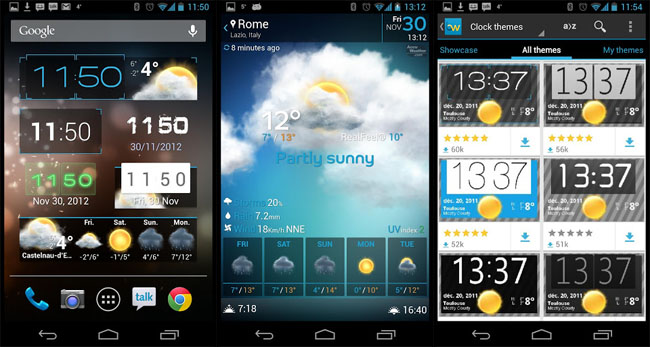
\includegraphics[scale=0.4]{widgets.jpg}
\end{center}
\end{frame}


\begin{frame}
\frametitle{Les types de widgets}
\begin{center}

\includegraphics[scale=0.5]{folders.jpg}
\end{center}
\begin{block}{Les différentes catégories de widgets sont :}
\begin{itemize}
\item Informations
\item Collection
\item Contrôle
\item Hybride
\end{itemize}
\end{block}
\end{frame}

\subsection{Widget d'informations}
\begin{frame}
\frametitle{Widgets d'information}
\begin{center}
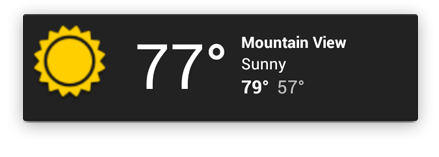
\includegraphics[scale=0.3]{widgets_info.png}
\end{center}

Ces widgets servent à afficher des informations utiles à l'utilisateur, et suivent leur évolution au cours du temps. De bons exemples sont les widgets météo, les horloges, les traqueurs de résultats sportifs...
\end{frame}

\subsection{Widgets de collection}
\begin{frame}
\frametitle{Widgets de collection}
\begin{center}
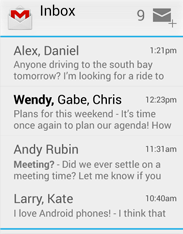
\includegraphics[scale=0.4]{widgets_collection_gmail.png}
\end{center}

Ils sont spécialisés dans l'affichage de collections d'éléments d'un même type, comme des collections d'e-mails, de messages, d'images ou encore d'articles. Ces widgets se concentrent sur deux opérations : parcourir la collection, et ouvrir un élément de la collection pour visualiser l'information complète (contenu d'un e-mail).
\end{frame}

\subsection{Widget de contrôle}
\begin{frame}
\frametitle{Widgets de contrôle}
\begin{center}
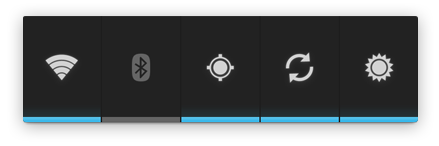
\includegraphics[scale=0.4]{widgets_control.png}
\end{center}

Le but des widgets de contrôle est de permettre l'utilisation rapide d'une fonction très utilisée depuis l'écran d'accueil, sans avoir besoin de lancer une application. Un exemple typique provient des lecteurs de musique, qui proposent de mettre en pause la lecture, ou de passer à la musique suivante sans devoir ouvrir l'application de lecture.
\end{frame}

\subsection{Widget de hybride}
\begin{frame}
\frametitle{Widgets hybrides}
\begin{center}
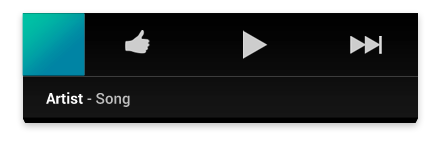
\includegraphics[scale=0.3]{widgets_hybrid.png}
\end{center}

La plupart des widgets rentrent dans une des catégories précédentes, mais il peut arriver que l'emploi de fonctions provenant de différentes catégories soit nécessaire. Dans ce cas, il est recommandé de se concentrer sur l'interface d'un des types précédent.

\begin{exampleblock}{Un lecteur de musique...}
...est avant tout un widget de contrôle, mais il permet aussi de suivre le nom du morceau lu, et utilise donc quelques composants d'un widget d'information.
\end{exampleblock}
\end{frame}

\begin{frame}
\frametitle{Mouvements}
\begin{center}
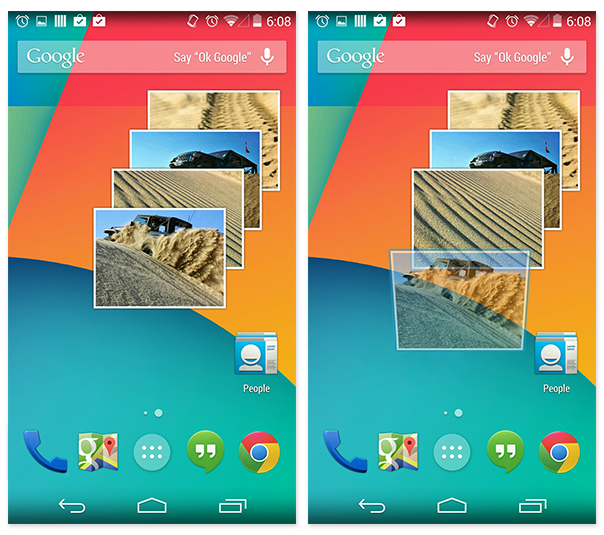
\includegraphics[scale=0.2]{widgets_gestures.png}
\end{center}
Du à leur contexte d'utilisation, les widgets sont techniquement 
limités pour ce qui est de leurs interaction avec l'utilisateur.
Par exemple, un widget présent sur l'écran d’accueil ne peut réagir 
qu'aux pressions de l'utilisateur et au slide vertical.
Le slide horizontal est déjà utilisé pour naviguer entre les
différents écrans d’accueil.
\end{frame}

\section{Créer un widget d'informations}
\begin{frame}
\frametitle{Créer un widget}
\begin{center}

\includegraphics[scale=0.4]{infos.jpg}
\end{center}
\end{frame}

\begin{frame}
\frametitle{Les RemoteViews}
\begin{center}

\includegraphics[scale=0.05]{remote.png}
\end{center}
\begin{block}{RemoteViews}
Les widgets vivent dans une application \emph{hôte} et il faut un mécanisme pour conserver les droits de l'application dont ils proviennent. Pour cela, leur vue est construite via des \verb!RemoteViews!. Les \verb!RemoteViews! conservent les droits de l'application \emph{invitée}.
\end{block}

\begin{block}{BroadcastReceiver}
Les interfaces sont construites par un \verb!BroadcastReceiver! qui produit les objets \verb!RemoteViews!. Cet objet est maintenu en vie par le système Android.
\end{block}
\end{frame}

\begin{frame}
\frametitle{Créer son widget}
\begin{center}

\includegraphics[scale=0.25]{todolist.png}
\end{center}
\begin{block}{Pour créer un widget, il faut :}
\begin{itemize}
\item Définir son layout
\item Créer un fichier XML (AppWidgetProviderInfo) qui décrit ses propriétés
\item Construire un BroadcastReceiver qui est utilisé pour construire l'interface du Widget.
\item Déclarer le widget dans le Manifest.
\item (Optionel) Ajouter une activité qui configure le widget.
\end{itemize}
\end{block}

\end{frame}

\subsection{Le layout}

\begin{frame}
\frametitle{Les éléments du layout}
\begin{center}
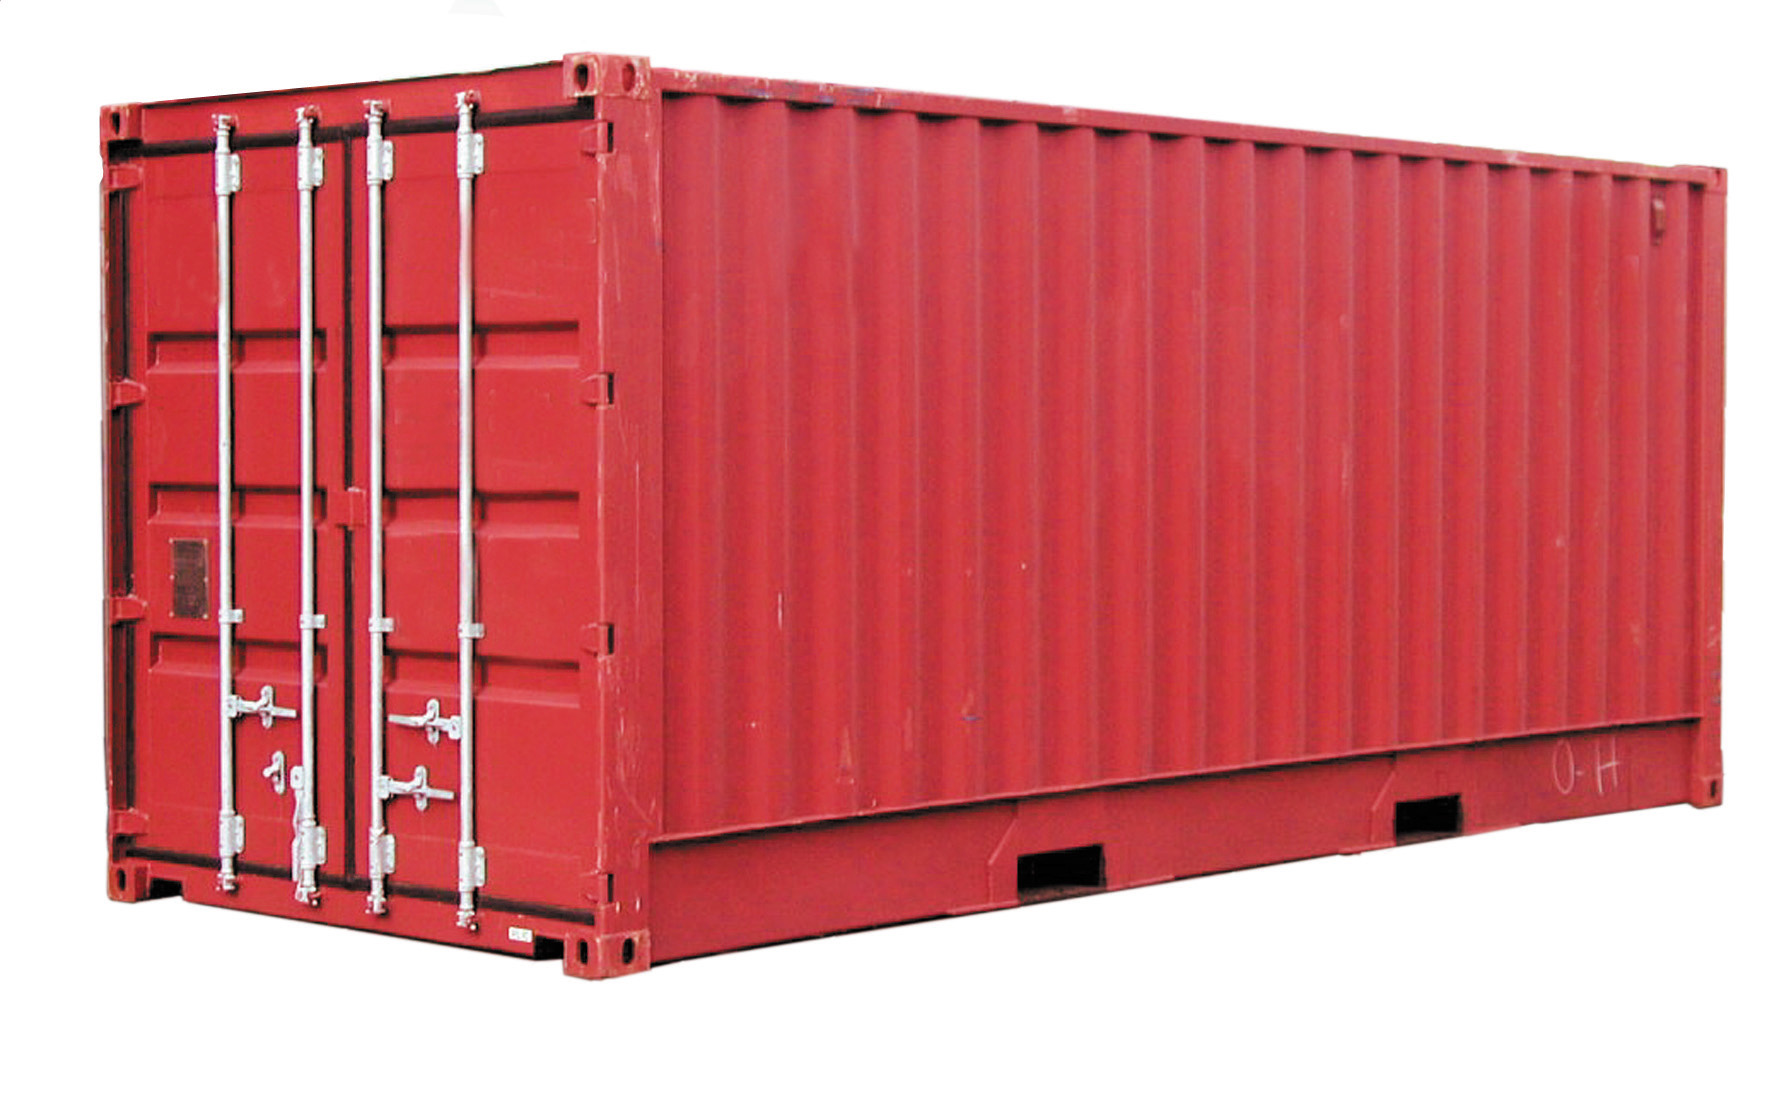
\includegraphics[scale=0.2]{container.jpg}
\end{center}
On ne peut utiliser que certains containers.
\begin{block}{Ne sont disponibles que les layouts :}
\begin{itemize}
\item FrameLayout
\item LinearLayout
\item RelativeLayout
\end{itemize}
\end{block}
\end{frame}

\begin{frame}
\frametitle{Les éléments du layout}
\begin{center}
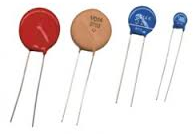
\includegraphics[scale=0.5]{comps.png}
\end{center}
On ne peut utiliser que certains composants graphiques.
\begin{block}{Seulement les composants suivants :}
\begin{itemize}
\begin{minipage}[t]{0.4\linewidth}
\item AnalogClock
\item Button
\item Chromometer
\item ImageButton
\end{minipage}
\begin{minipage}[t]{0.4\linewidth}
\item ImageView
\item ProgressBar
\item TextView
\end{minipage}
\end{itemize}
\end{block}
\end{frame}

\begin{frame}
\frametitle{Mon Layout}
Par la suite, on supposera avoir décrit l'apparence de notre widget dans un fichier \verb!mywidget\_layout.xml!.
\end{frame}


\begin{frame}
\frametitle{Les actions disponibles}
\begin{center}

\includegraphics[scale=0.35]{listener.jpg}
\end{center}
\begin{block}{OnClickListener}
La seul interaction possible avec la vue s'effectue via un \verb!OnClickListener!. Ce listener peut être lié à un \emph{composant graphique} et déclenché par l'utilisateur au moment du clic sur ce \emph{composant}.
\end{block}
\end{frame}

\subsection{Le XML descriptif}

\begin{frame}[fragile]
\frametitle{Description du Widget}

\begin{exampleblock}{On crée un fichier \verb!mywidget\_info.xml! dans \verb!/res/xml/! contenant : }
\lstset{language=xml}
\begin{lstlisting}
<appwidget-provider xmlns:android="http://schemas.android.com/apk/res/android"
    android:minWidth="40dp"
    android:minHeight="40dp"
    android:updatePeriodMillis="86400000"
    android:previewImage="@drawable/preview"
    android:initialLayout="@layout/mywidget_layout"
    android:resizeMode="horizontal|vertical"
    android:widgetCategory="home_screen">
</appwidget-provider>
\end{lstlisting}
\end{exampleblock}
\end{frame}

\begin{frame}[fragile]
\frametitle{Description du Widget}

\begin{exampleblock}{Si on veut une activité de configuration : }
\lstset{language=xml}
\begin{lstlisting}
<appwidget-provider xmlns:android="http://schemas.android.com/apk/res/android"
    ...
    android:configure="com.example.android.MyWidgetConfigure">
</appwidget-provider>
\end{lstlisting}
\end{exampleblock}

\begin{block}{}
Cette ligne indique la classe correspondant à l'activité qui doit être exécutée.
\end{block}
\end{frame}

\begin{frame}
\frametitle{Description du Widget}
\begin{block}{Description des attributs.}
\begin{itemize}
\item \verb!minWidth! et \verb!minHeight! contrôlent la taille minimale,
\item \verb!updatePeriodMillis! définit le temps de rafraichissement,
\item \verb!initialLayout! indique le layout de votre widget,
\item \verb!reviewImage! indique l'image qui sera affichée dans la liste des widgets,
\item \verb!resizeMode! indique dans quelles directions on peut redimensionner le widget,
\item \verb!widgetCategory! indique dans quelle zone le widget peut être placé (home\_screen et keyguard).
\end{itemize}
\end{block}
\end{frame}

\subsection{Le provider}

\begin{frame}[fragile]
\frametitle{La classe provider}
On ajoute une nouvelle classe \verb!MyWidgetProvider! chargée de construire les vues.
\begin{exampleblock}{Notre classe provider :}
\lstset{language=java}
\begin{lstlisting}
public class MyWidgetProvider extends AppWidgetProvider {

    public void onUpdate(Context context, AppWidgetManager appWidgetManager, int[] appWidgetIds) {
        //Effectue la mise a jour de la vue
    }
\end{lstlisting}
\end{exampleblock}
\end{frame}


\begin{frame}[fragile]
\frametitle{La fonction \verb!onUpdate!}
\begin{center}

\includegraphics[scale=1]{update.jpg}
\end{center}
\begin{block}{Les arguments de cette fonction sont :}
\begin{itemize}
\item[] {\color{blue} \verb!context!} -- Informations sur votre application,
\item[] {\color{blue} \verb!appWidgetManager!} -- Le gestionnaire de widgets,
\item[] {\color{blue} \verb!appWidgetIds!} -- La liste de toutes les instances de notre widget.
\end{itemize}
\end{block}
\end{frame}

\begin{frame}[fragile]
\frametitle{La fonction \verb!onUpdate!}
\begin{block}{Implémentation de \verb!onUpdate!}
\lstset{language=java}
\begin{lstlisting}
// On parcourt tous les widgets.
final int N = appWidgetIds.length;
for (int i = 0; i < N; i++) {
    int appWidgetId = appWidgetIds[i];

    //Construit une nouvelle vue.
    RemoteViews views = new RemoteViews(context.getPackageName(), R.layout.mywidget_layout);

    // Change le contenu du champ text textField.
    views.setTextViewText(R.id.textField, "Blabla");

    // Met a jour la vue avec notre nouvelle vue.
    appWidgetManager.updateAppWidget(appWidgetId, views);
}
\end{lstlisting}
\end{block}
\end{frame}

\subsection{Le manifest}
\begin{frame}[fragile]
\begin{block}{On déclare le provider dans le block \verb!<application></application>!.}
\lstset{language=xml}
\begin{lstlisting}
<receiver android:name="MyWidgetProvider" >
    <intent-filter>
        <action android:name="android.appwidget.action.APPWIDGET_UPDATE" />
    </intent-filter>

    <meta-data
        android:name="android.appwidget.provider"
        android:resource="@xml/mywidget_info" />
</receiver>
\end{lstlisting}
\end{block}
\end{frame}

\subsection{Réagir a un clic}
\begin{frame}
\frametitle{L'intent ACTION\_APPWIDGET\_UPDATE}
\begin{block}{Une pending intent}
C'est une intention qui est conservé un certain laps de temps avant d’être envoyé au système. Les données qu'elle contient sont conservées aussi longtemps que l'intent existe.
\end{block}
\begin{block}{ACTION\_APPWIDGET\_UPDATE}
L'intention \verb!ACTION\_APPWIDGET\_UPDATE! permet de mettre à jour la vue d'un widget en provoquant l'appel à \verb!onUpdate!.
\end{block}
\end{frame}

\begin{frame}[fragile]
\lstset{language=java}
\begin{block}{Lier un clic à une mise à jours (dans onUpdate)}
\begin{lstlisting}
// Creation de notre intention
Intent intent = new Intent();

//Intent de type mise a jour de widget
intent.setAction(AppWidgetManager.ACTION_APPWIDGET_UPDATE);
//On dit quel widget on veut mettre a jour
intent.putExtra(AppWidgetManager.EXTRA_APPWIDGET_IDS, appWidgetIds);

//Si l'intent existe deja, on la met juste a jour.
PendingIntent pendingIntent = PendingIntent.getBroadcast(
    context, 0, intent, PendingIntent.FLAG_UPDATE_CURRENT);
remoteViews.setOnClickPendingIntent(R.id.button, pendingIntent);
\end{lstlisting}
\end{block}
\end{frame}
\subsection{Configurer un widget}
\begin{frame}
\frametitle{Activité de configuration}
\begin{center}

\includegraphics[scale=0.3]{config.png}
\end{center}
\end{frame}

\begin{frame}[fragile]
\frametitle{L'activité de configuration}
\begin{block}{L'activité sera lancée par une intent}
\lstset{language=xml}
\begin{lstlisting}
<activity android:name=".ExampleAppWidgetConfigure">
    <intent-filter>
        <action android:name="android.appwidget.action.APPWIDGET_CONFIGURE"/>
    </intent-filter>
</activity>
\end{lstlisting}
\end{block}
\begin{block}{Et elle doit aussi être spécifiée au provider}
\begin{lstlisting}
<appwidget-provider xmlns:android="http://schemas.android.com/apk/res/android"
    ...
    android:configure="com.example.android.ExampleAppWidgetConfigure" 
    ... >
</appwidget-provider>
\end{lstlisting}
\end{block}
\end{frame}

\begin{frame}
\frametitle{Bon à savoir...}
\begin{itemize}
\item L'application de configuration doit toujours renvoyer un résultat. Ce résultat doit inclure l'ID du widget obtenu par l'application de configuration à travers le champ \verb!EXTRA\_APPWIDGET\_ID!.
\item La fonction onUpdate n'est pas appelée lors de la création du widget. Ce sera à l'application de configuration de provoquer son appel.
\end{itemize}

\end{frame}

\begin{frame}[fragile]
\frametitle{Step by step...}

\begin{block}{1 - Récupérer l'ID de l'App Widget}
\begin{lstlisting}
Intent intent = getIntent();
Bundle extras = intent.getExtras();
if (extras != null) {
    mAppWidgetId = extras.getInt(
            AppWidgetManager.EXTRA_APPWIDGET_ID, 
            AppWidgetManager.INVALID_APPWIDGET_ID);
}
\end{lstlisting}
\end{block}

\begin{block}{2 - Configuration}
Faites ce que vous avez à faire dans votre activité.
\end{block}
\end{frame}

\begin{frame}[fragile]
\frametitle{Step by step...}

\begin{block}{3 - Récupérer le manager}
\begin{lstlisting}
AppWidgetManager appWidgetManager = AppWidgetManager.getInstance(context);
\end{lstlisting}
\end{block}

\begin{block}{4 - Mettre à jour le widget}
\begin{lstlisting}
RemoteViews views = new RemoteViews(context.getPackageName(),
R.layout.example_appwidget);
appWidgetManager.updateAppWidget(mAppWidgetId, views);
\end{lstlisting}
\end{block}

\end{frame}

\begin{frame}[fragile]
\frametitle{Step by step...}

\begin{block}{5 - Ajouter le résultat et terminer l'activité}
\begin{lstlisting}
Intent resultValue = new Intent();
resultValue.putExtra(AppWidgetManager.EXTRA_APPWIDGET_ID, mAppWidgetId);
setResult(RESULT_OK, resultValue);
finish();
\end{lstlisting}
\end{block}

\begin{block}{Conseil :}
Créez l'intent de résultat dès le début de l'activité, avec la valeur \verb!RESULT_CANCELED!, et liez-la avec \verb!setResult()!. De cette façon, si l'utilisateur quitte l'activité de configuration avec le bouton back, le widget ne sera pas créé.
\end{block}

\end{frame}


\section{Conclusion}

\begin{frame}
\begin{center}
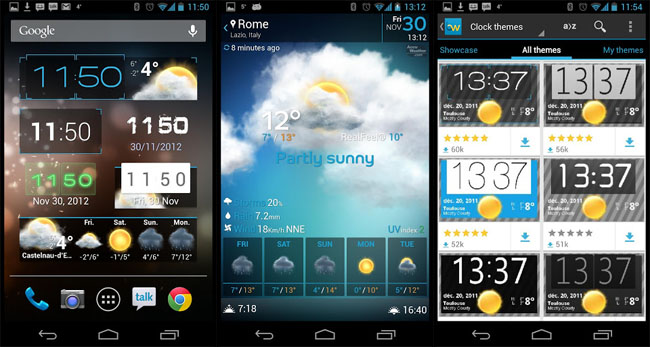
\includegraphics[scale=0.3]{widgets.jpg}
\end{center}
\begin{block}{Widgets}
Avec un widget, vous pouvez enrichir vos application et proposer à vos utilisateurs le suivi d'un monitoring sportif, l'affichage de données agrégées, les derniers messages reçus sur une application sociale, etc.
\end{block}

\end{frame}

\begin{frame}
\begin{center}
Pour me contacter : jeremy.cochoy@gmail.com, merci et à bientôt.

\medskip
\medskip
\medskip
\medskip


\includegraphics[scale=0.3]{android_cat.jpg}
\end{center}
\end{frame}




\end{document}